\documentclass[journal]{IEEEtran}
\usepackage{cite}
\usepackage{amsmath,amssymb,amsfonts}
\usepackage{graphicx}
\usepackage{booktabs}
\usepackage{multirow}
\usepackage{siunitx}
\usepackage{xcolor}
\usepackage{url}
\usepackage[hidelinks]{hyperref}
\graphicspath{{../figures/}}
\newcommand{\fop}{1.000}
\newcommand{\fs}{950.0}
\newcommand{\Cnought}{1.20}
\newcommand{\Cm}{0.30}
\newcommand{\Cratio}{0.25}
\newcommand{\kt}{24.7}
\newcommand{\Qm}{500}
\newcommand{\Lm}{93.6}
\newcommand{\Rm}{1.12}
\newcommand{\fp}{1062.1}
\newcommand{\Csh}{3.91}
\newcommand{\Csw}{7.78}
\newcommand{\Cpar}{0.00}
\newcommand{\Wsw}{1865}
\newcommand{\Ron}{0.19}
\newcommand{\Coff}{1119}
\newcommand{\Qsw}{109}
\newcommand{\xratio}{0.04}
\newcommand{\fm}{40.0}
\newcommand{\fclk}{240}
\newcommand{\clockratio}{4.2}
\newcommand{\ILdB}{0.00}
\newcommand{\ISOdB}{0.00}
\newcommand{\RLdB}{0.00}
\newcommand{\IMup}{0.00}
\newcommand{\IMdn}{0.00}
\newcommand{\Pmod}{0.00}
\newcommand{\Pcore}{0.00}
\newcommand{\Pmodtot}{0.00}
\newcommand{\phasetwo}{0.00}
\newcommand{\phasethree}{0.00}
\newcommand{\phaseerr}{0.1}
\newcommand{\trise}{0.00}
\newcommand{\trisepct}{0.0}
\newcommand{\agreeIL}{0.01}
\newcommand{\agreeISO}{0.1}
\newcommand{\idealIL}{0.00}
\newcommand{\idealISO}{0.00}
\newcommand{\BWisong}{0.00}
\newcommand{\ILltp}{3.03}
\newcommand{\ISOltp}{22.8}
\newcommand{\RLltp}{11.9}
\newcommand{\BWiso}{2.38}
\newcommand{\BWisofifteen}{6.38}
\newcommand{\BWil}{7.62}
\newcommand{\BWrl}{5.00}
\newcommand{\revIL}{22.77}
\newcommand{\revISO}{3.0}
\newcommand{\fdeg}{979.2}
\newcommand{\Qload}{44}
\newcommand{\bwdeg}{22.5}
\newcommand{\Sunmod}{-4.6}
\newcommand{\Sunmodrl}{15.0}
\newcommand{\Qe}{0.00}
\newcommand{\Qi}{0.00}
\newcommand{\kappaMHz}{0.0}
\newcommand{\dfMHz}{0.0}
\newcommand{\dfused}{0.0}
\newcommand{\slope}{0.00}
\newcommand{\geMHz}{0.00}
\newcommand{\wmratio}{40000000.0}
\newcommand{\dwratio}{0.0}
\newcommand{\kratio}{0.0}
\newcommand{\lossratio}{0.00}
\newcommand{\fomval}{0.0}
\newcommand{\gzerophase}{-102}
\newcommand{\fonres}{997.0}
\newcommand{\geon}{18.3}
\newcommand{\gion}{7.9}
\newcommand{\Qeon}{27}
\newcommand{\Qion}{63}
\newcommand{\geoff}{5.8}
\newcommand{\detoff}{29}
\newcommand{\detoffhalf}{15}
\newcommand{\lossratioon}{0.43}
\newcommand{\cmtilpred}{3.7}
\newcommand{\phasetol}{10}
\newcommand{\cswtol}{10}
\newcommand{\Pmaxone}{-3.1}
\newcommand{\Pmaxtwo}{2.9}
\newcommand{\vdspk}{0.24}
\newcommand{\Pinng}{-7.0}
\newcommand{\projILq}{2.14}
\newcommand{\projILbest}{1.73}
\newcommand{\vdspkpervolt}{2.7}
\newcommand{\chanw}{108}
\newcommand{\chanh}{116}
\newcommand{\cmtrows}{2 & 2.7 & 2.80 & 3.01 & 12.0 \\
3 & 4.2 & 3.02 & 1.85 & 15.1 \\
4 & 5.9 & 3.30 & 1.34 & 17.7 \\
5 & 7.9 & 3.58 & 1.04 & 20.0 \\
7 & 10.1 & 4.15 & 0.75 & 21.6 \\
10 & 12.0 & 4.82 & 0.53 & 24.4 \\
15 & 12.0 & 5.59 & 0.39 & 25.9 \\}
\newcommand{\projrows}{500 & 350 & 2.83 & 19.6 & 14.4 & 0.0 \\
500 & 200 & 2.80 & 19.6 & 14.5 & 0.0 \\
500 & 100 & 2.78 & 19.7 & 14.5 & 0.0 \\
1000 & 350 & 2.14 & 21.0 & 16.0 & 2.0 \\
1000 & 200 & 2.11 & 21.1 & 16.1 & 2.0 \\
1000 & 100 & 2.09 & 21.2 & 16.2 & 2.0 \\
2000 & 350 & 1.79 & 21.9 & 17.0 & 2.0 \\
2000 & 200 & 1.75 & 22.0 & 17.1 & 2.0 \\
2000 & 100 & 1.73 & 22.1 & 17.1 & 2.0 \\}
\newcommand{\toporows}{A: parallel-mode loop & A-MOS varactor & 5.30 & 5.3 & 15.0 & 9.9 \\
C: series-mode junction & A-MOS varactor & 4.92 & 29.5 & 7.9 & 16.5 \\
C: series-mode junction & switched MIM & 3.19 & 30.2 & 10.5 & 41.0 \\
C, $Q_m=1000$ & switched MIM & 2.39 & 30.0 & 12.4 & 38.0 \\}
\newcommand{\varIL}{4.92}
\newcommand{\varISO}{29.5}
\newcommand{\loopIL}{5.30}
\newcommand{\loopISO}{5.3}

\sisetup{detect-all}

\begin{document}
\title{A CMOS-Driven Nonreciprocal Acoustic Circulator Based on Spatiotemporal Modulation of a Lithium-Niobate Resonant Junction for Full-Duplex RF Front-Ends}

\author{M.~Nisha~Angeline,~\IEEEmembership{Senior Member,~IEEE}%
\thanks{M. Nisha Angeline is with the Department of Electronics and Communication Engineering, Velalar College of Engineering and Technology, Thindal, Erode, Tamil Nadu, India (e-mail: nishavlsidesign@gmail.com).}%
\thanks{Manuscript prepared October 2026. All results in this paper are simulation results (transistor-level transient co-simulation in ngspice and a conversion-matrix periodic S-parameter analysis equivalent to Spectre PSS/PSP); no device has been fabricated or measured.}}

\markboth{IEEE Transactions on Microwave Theory and Techniques}{Nisha Angeline: CMOS-Driven Nonreciprocal Acoustic Circulator}

\maketitle

\begin{abstract}
Ferrite circulators are the only component of a full-duplex radio front-end that has resisted integration. Magnet-free CMOS alternatives based on switched networks are integrated but require multi-phase clocks at the carrier frequency and tens of milliwatts, while lumped-element spatiotemporally modulated (STM) circulators need off-chip inductors. This paper presents the co-design of a chip-scale circulator in which three lithium-niobate (LiNbO$_3$) laterally vibrating resonators form a series-mode resonant junction whose branches are modulated by switched MIM capacitors driven with \ang{0}/\ang{120}/\ang{240} phases from a \SI{65}{nm} CMOS divide-by-six Johnson counter. A Floquet coupled-mode theory gives closed-form design rules for angular-momentum-biased resonator loops and shows that the loss-limited insertion loss of any STM acoustic circulator is set by a single tunability--quality-factor product $Q_t\,\Delta f/f_0$; the same analysis explains why the classical capacitively coupled parallel-mode loop cannot be realised with acoustic resonators (the ring coupling collapses the tunability), which motivates the junction topology in which the in-phase mode is made non-resonant by the floating star node. The design is verified with a conversion-matrix periodic S-parameter solver (the analysis Spectre performs with PSS+PSP, validated to \SI{0.01}{dB} against analytic sideband theory) and with transistor-level transient co-simulation of the complete chip in ngspice with a \SI{65}{nm} BSIM4 model. At \SI{\fop}{GHz} the complete design achieves \SI{\ILdB}{dB} insertion loss, \SI{\ISOdB}{dB} isolation and \SI{\RLdB}{dB} return loss with a \SI{\BWiso}{MHz} 20-dB isolation bandwidth; the pump at \SI{\fm}{MHz}, \num{\clockratio} times below the carrier, consumes \SI{\Pmodtot}{mW} and the device contains no inductor.  Spectre netlists, an OCEAN PSS/PSP script, SKILL schematic generators and a tape-out candidate GDSII layout are provided for reproduction in Cadence Virtuoso.
\end{abstract}

\begin{IEEEkeywords}
Acoustic resonators, circulators, full-duplex, lithium niobate, magnet-free nonreciprocity, MEMS, spatiotemporal modulation, switched capacitors, time-varying circuits.
\end{IEEEkeywords}

\IEEEpeerreviewmaketitle

\section{Introduction}
\IEEEPARstart{I}{n-band} full-duplex (IBFD) radios transmit and receive simultaneously in the same channel and can, in principle, double spectral efficiency \cite{sabharwal2014inband,bharadia2013full,zhou2017integrated}. The first and most demanding stage of the self-interference cancellation chain is the antenna interface: a three-port circulator that routes the transmitter to the antenna and the antenna to the receiver while isolating the receiver from the transmitter. Ferrite junction circulators perform this function with \SIrange{0.3}{0.6}{dB} insertion loss but rely on a permanent magnet and a centimetre-scale garnet puck, and remain the only front-end component that has not been integrated \cite{kord2020microwave,caloz2018electromagnetic}.

Time modulation breaks reciprocity without magnets \cite{sounas2017nonreciprocal,nagulu2020nonreciprocal}. Two families have emerged. In \emph{commutated} (N-path or switched-delay-line) circulators \cite{reiskarimian2016magnetic,reiskarimian2017cmos,dinc2017synchronized,dinc2017millimeter,nagulu2019nonmagnetic,biedka2017ultra}, CMOS switches are clocked at or near the carrier frequency; they are fully integrated but need multi-phase clocks at the RF frequency with clock power in the tens of milliwatts, together with transmission-line or lumped delay elements. In \emph{spatiotemporally modulated} (STM) resonator circulators \cite{sounas2013giant,estep2014magnetic,kord2018magnetless,kord2018pseudo,kord2018broadband,kord2019magnetless,qin2014nonreciprocal}, three resonators arranged with three-fold symmetry are modulated with phases of \ang{0}, \ang{120} and \ang{240}; the pump frequency is a small fraction of the carrier, but the demonstrations used printed inductors and the attainable loss is bounded by the inductor quality factor ($Q\!\approx$ 10--30 on chip). Acoustic implementations replace the inductors with piezoelectric resonators whose $Q$ is one to two orders of magnitude higher: sound circulators with moving media \cite{fleury2014sound,fleury2015subwavelength}, commutated FBAR \cite{torunbalci2018fbar} and MEMS-resonator \cite{yu2018magnetic,yu2019highly} circulators, STM SAW-filter circulators \cite{yu2019radio} and nonlinear parity--time-symmetric microwave acoustic devices \cite{shao2020nonreciprocal}. These demonstrations used bench signal generators as the pump and did not address the co-design of the modulating electronics, nor the question of which resonator topology is compatible with the limited frequency tunability of an acoustic resonator.

This paper addresses both. The contributions are:
\begin{enumerate}
\item a Floquet coupled-mode theory (CMT) of frequency-modulated three-resonator loops that yields normalised design rules ($\kappa/\gamma_e$, $\Delta\omega/\gamma_e$, $\omega_m/\gamma_e$) and a closed-form loss scaling in terms of the tunability--quality-factor product of the modulated resonator (Section~\ref{sec:theory});
\item the finding, from circuit-exact analysis, that the capacitively coupled parallel-mode loop of \cite{estep2014magnetic} cannot be realised with acoustic resonators because the ring-coupling capacitors multiply the susceptance slope of the resonator and destroy its tunability, and the series-mode resonant junction (wye) that solves the problem by making the in-phase mode non-resonant without any coupling element (Section~\ref{sec:arch});
\item a switched-MIM modulator (a two-state ``digital varactor'' made of a MIM capacitor and a wide nMOS switch) that out-performs the analogue accumulation-mode varactor in both quality factor and pump power (Section~\ref{sec:arch});
\item the \SI{65}{nm} CMOS pump: a divide-by-six Johnson counter that generates exactly \ang{120}-spaced phases from a single reference clock, tapered gate drivers and a direction-reversal option (Section~\ref{sec:cmos});
\item a two-level verification flow, conversion-matrix periodic S-parameters and transistor-level transient co-simulation, cross-checked against each other and against the CMT (Sections~\ref{sec:method} and \ref{sec:results}); and
\item Cadence Virtuoso deliverables (Spectre netlists, OCEAN PSS/PSP script, SKILL schematic generators) and a tape-out candidate GDSII layout (Section~\ref{sec:layout}).
\end{enumerate}
All results are simulated; the paper is a complete design study whose files allow the design to be transferred to a foundry PDK.

\section{Operating Principle and Coupled-Mode Theory}\label{sec:theory}
\subsection{Floquet CMT of an angular-momentum-biased loop}
Consider three identical resonators with amplitudes $a_n(t)$, $n=0,1,2$, coupled to their neighbours with rate $\kappa$ and each to a \SI{50}{\ohm} port with external decay rate $\gamma_e$; $\gamma_i$ is the intrinsic decay rate. The resonance frequency of each resonator is modulated,
\begin{equation}
\omega_n(t)=\omega_0+\Delta\omega\, m(\omega_m t-2\pi n/3),
\label{eq:mod}
\end{equation}
with $m(\theta)=\cos\theta$ (sinusoidal pump) or $m(\theta)=\mathrm{sgn}\cos\theta$ (square-wave pump), so that the modulation carries one quantum of angular momentum around the loop \cite{sounas2013giant,estep2014magnetic}. The temporal CMT equations are
\begin{align}
\dot a_n &= \left[j\omega_n(t)-\gamma_i-\gamma_e\right]a_n + j\kappa\,(a_{n+1}+a_{n-1}) + \sqrt{2\gamma_e}\,s^{+}_n,\label{eq:cmt1}\\
s^{-}_n &= -s^{+}_n + \sqrt{2\gamma_e}\,a_n,\label{eq:cmt2}
\end{align}
with incident and reflected waves $s^{\pm}_n$. Because the coefficients are periodic, an input at $\omega$ produces a response at all $\omega+k\omega_m$. Expanding $a_n(t)=\sum_k A_{n,k}e^{j(\omega+k\omega_m)t}$ turns (\ref{eq:cmt1}) into a linear system in the harmonic index $k$ (truncated at $|k|\le K$) whose solution gives the scattering matrix at the fundamental, $S_{mn}(\omega)$, and the sideband conversion gains $S^{(k)}_{mn}(\omega)$. We solve it exactly, without rotating-wave or small-modulation approximations, for $K=6$--$8$.

In the basis of loop modes with angular momentum $l\in\{0,\pm1\}$ the unmodulated loop has eigenfrequencies $\omega_l=\omega_0+2\kappa\cos(2\pi l/3)$: a non-degenerate mode at $\omega_0+2\kappa$ and a degenerate counter-rotating pair at $\omega_0-\kappa$. Since angular momentum is defined modulo three, the first-order modulation couples $|{+1},k\rangle\leftrightarrow|{-1},k{+}1\rangle$ and $|{-1},k\rangle\leftrightarrow|{+1},k{-}1\rangle$ with coupling $\Delta\omega/2$ and detuning $\pm\omega_m$. For $\omega_m\gg\gamma_e$ this off-resonant coupling produces second-order shifts of opposite sign on the two counter-rotating modes, i.e.\ an effective angular-momentum bias that splits them by
\begin{equation}
\delta\approx\frac{\Delta\omega^2}{2\omega_m}.
\label{eq:split}
\end{equation}
Exactly as in a ferrite junction circulator, perfect circulation requires the reflection phases of the three eigenmodes to be spaced by \ang{120}; with the $l=0$ mode far detuned or non-resonant, this is obtained when $\delta=2\gamma_e\tan\ang{30}\approx1.15\gamma_e$, i.e.\ $\Delta\omega\approx\sqrt{2.3\,\gamma_e\omega_m}$.

\subsection{Normalised design rules}
Table~\ref{tab:cmt} lists the optimum of (\ref{eq:cmt1})--(\ref{eq:cmt2}) found by a global search over $\kappa$, $\Delta\omega$ and the operating frequency for several pump frequencies, with a target isolation of \SI{35}{dB}. The scaling of (\ref{eq:split}) is reproduced ($\Delta\omega/\gamma_e\!\approx\!1.5\sqrt{\omega_m/\gamma_e}$), the optimum always places the $l=0$ mode $3|\kappa|\ge 20\gamma_e$ away from the pair, and the lossless insertion loss falls monotonically with $\omega_m/\gamma_e$ because the intermodulation sidebands at $\omega\pm\omega_m$ move out of the resonator bandwidth: \SI{3.0}{dB} at $\omega_m=2\gamma_e$, \SI{1.0}{dB} at $5\gamma_e$ and \SI{0.4}{dB} at $15\gamma_e$. Square-wave (CMOS) modulation with the same fundamental amplitude costs less than \SI{0.1}{dB} and \SI{1}{dB} of isolation because its third harmonic carries zero net angular momentum and its fifth is \SI{14}{dB} weaker.

\begin{table}[!t]
\centering
\caption{Normalised CMT optimum (lossless, isolation target 35 dB)}
\label{tab:cmt}
\footnotesize
\begin{tabular}{S[table-format=2.0] S[table-format=2.1] S[table-format=1.2] S[table-format=1.2] S[table-format=2.1]}
\toprule
{$\omega_m/\gamma_e$} & {$|\kappa|/\gamma_e$} & {$\Delta\omega/\gamma_e$} & {IL (dB)} & {RL (dB)}\\
\midrule
\cmtrows
\bottomrule
\end{tabular}
\end{table}

\subsection{Loss scaling and the tunability--$Q$ product}
With intrinsic loss the CMT insertion loss depends only on $\gamma_i/\gamma_e$: \SI{1.2}{dB} at $\gamma_i/\gamma_e=0.1$, \SI{2.0}{dB} at $0.2$, \SI{2.8}{dB} at $0.3$ and \SI{4.2}{dB} at $0.5$ (with the isolation degrading from \SI{35}{} to \SI{18}{dB} over the same range). Because the design rules fix $\Delta\omega=c\,\gamma_e$ with $c\approx3.3$--$5.6$ for $\omega_m=4$--$15\gamma_e$, and because the available peak frequency deviation of the fundamental of the pump waveform is $\Delta f$,
\begin{equation}
\frac{\gamma_i}{\gamma_e}=\frac{\omega_0/(2Q_t)}{\Delta\omega/c}=\frac{c}{2}\,\frac{1}{Q_t\,\Delta f/f_0},
\label{eq:fom}
\end{equation}
where $Q_t$ is the quality factor of the modulated resonator (acoustic resonator and modulator together). Equation (\ref{eq:fom}) is the central design constraint of any STM acoustic circulator: an insertion loss below \SI{2}{dB} requires $Q_t\,\Delta f/f_0\gtrsim 10$--$14$. An on-chip LC tank ($Q_t\!\approx\!15$) needs a \SI{100}{\percent} tuning range; an acoustic resonator with $Q_t\!\approx\!500$ needs only \SI{3}{\percent}, but as shown next the topology decides whether this \SI{3}{\percent} is available.

\section{Circuit Architecture}\label{sec:arch}
\subsection{Acoustic resonator model}
The resonators are X-cut LiNbO$_3$ shear-horizontal (SH0) laterally vibrating resonators \cite{gong2013design,lu2018lithium}, chosen for their electromechanical coupling ($k_t^2\approx$ \SIrange{20}{25}{\percent}) which sets the separation between series and parallel resonance and therefore the tuning range. Each resonator is described by the modified Butterworth--Van~Dyke (mBVD) model \cite{larson2000modified}: $C_0=\SI{\Cnought}{pF}$, $C_m=\SI{\Cm}{pF}$ ($C_m/C_0=\Cratio$, $k_t^2=\SI{\kt}{\percent}$), $Q_m=\Qm$, $R_s=\SI{0.5}{\ohm}$, $R_0=\SI{0.3}{\ohm}$, giving $L_m=\SI{\Lm}{nH}$ and $R_m=\SI{\Rm}{\ohm}$ at $f_s=\SI{\fs}{MHz}$ ($f_p=\SI{\fp}{MHz}$). These values are representative of published \SI{1}{GHz}-class devices; they are parameters of the model, not measurements.

\subsection{Why the parallel-mode loop fails with acoustic resonators}
The natural translation of the lumped STM loop \cite{estep2014magnetic} replaces each LC tank by a resonator at its parallel resonance $f_p$, adds a shunt varactor, couples the ports through series capacitors $C_p$ and the tanks through a ring of capacitors $C_c$. Three properties of a piezoelectric resonator defeat this translation. First, at $f_p$ the susceptance slope is dominated by the motional branch, $dB/d\omega\approx 2L_m\omega^2C_{\rm tot}^2\gg C_{\rm tot}$ (\SI{89}{pF} for $C_{\rm tot}=\SI{2.8}{pF}$ in our resonator against \SI{2.8}{pF} for an LC tank), so a given $\kappa$ needs a ring capacitor $C_c$ that is \SI{30}{} times larger than for an LC loop. Second, the ring capacitors add $3C_c$ to the counter-rotating modes, which moves them towards $f_s$ where the slope grows as $C_{\rm tot}^2$: in the circuit of Section~\ref{sec:method} the loaded $Q$ of the counter-rotating pair doubles (\SI{216}{} against \SI{108}{} for the in-phase mode) and the tuning sensitivity $df/dC_v\propto C_m/C_{\rm tot}^2$ collapses by an order of magnitude. Third, the varactor loads the tank with its own conductance. The result is $Q_t\Delta f/f_0\approx 2$--$3$, i.e.\ $\gamma_i/\gamma_e\approx1$ in (\ref{eq:fom}): a global search over $C_p$, $C_c$, varactor size, swing and pump frequency with an adaptive operating frequency never found better than \SI{\loopIL}{dB} insertion loss with \SI{\loopISO}{dB} isolation (Table~\ref{tab:topo}). This is a general conclusion, independent of the specific resonator: capacitive ring coupling and capacitive tuning compete for the same susceptance budget.

\subsection{Series-mode resonant junction}
Fig.~\ref{fig:core} shows the topology adopted instead. Each port is matched by a shunt MIM capacitor $C_{sh}$ and feeds a series branch consisting of the resonator, the modulated capacitor and the switch; the three branches meet at a floating star node. For the counter-rotating modes ($l=\pm1$) the branch currents sum to zero at the star, which is therefore a virtual ground, and each branch is a series resonator between its port and ground with resonance between $f_s$ and $f_p$ set by the series capacitance. For the in-phase mode ($l=0$) the star carries no current and the branch is open: the $l=0$ mode is non-resonant and plays the role of the far-detuned mode of Table~\ref{tab:cmt} without any coupling element. The shunt $C_{sh}$ transforms the port resistance down to $R'=R_0/(1+(\omega C_{sh}R_0)^2)$ and sets $\gamma_e$; the series modulated capacitance $C_v$ in series with $C_m$ tunes the branch with sensitivity $\Delta f/f\approx (C_m/C_v)\,\Delta C_v/(2C_v)$, which for $C_m/C_v\approx\xratio$ gives several percent and keeps the $l=\pm1$ pair below $f_p$. Unlike the parallel loop, the junction has no element that competes with the tuning, and the whole device contains only capacitors, resistors, acoustic resonators and transistors.

\subsection{Modulator: switched MIM capacitor versus A-MOS varactor}
Two modulators were compared with the same resonator and the same global search. The accumulation-mode MOS varactor \cite{andreani2000use} ($C_{\max}/C_{\min}=2.5$, $Q_v\approx75$ at \SI{1}{GHz}) reaches $Q_t\Delta f/f_0\approx5$ and \SI{\varIL}{dB} insertion loss (Table~\ref{tab:topo}). The switched MIM capacitor of Fig.~\ref{fig:driver}, a MIM capacitor $C_{sw}=\SI{\Csw}{pF}$ in series with an nMOS switch of total width $W=\SI{\Wsw}{\micro\meter}$, toggles the branch between a resonant state (switch on, $R_{on}=\SI{\Ron}{\ohm}$) and a detuned state (switch off, where the gate and junction capacitances of the switch appear as a series capacitance $C_{off}=\SI{\Coff}{fF}$ and move the branch resonance above $f_p$); the modulation depth is no longer small, which the exact Floquet solver handles without approximation.

The switch is used in the standard RF-switch configuration: the gate is driven through $R_g=\SI{3}{k\ohm}$ so that it floats at RF, and the triple-well body is tied to the source through $R_b=\SI{20}{k\ohm}$. This matters more here than in an ordinary series switch: the source terminals of the three switches form the star node, and any parasitic capacitance from the star to ground destroys the open-circuit condition that makes the in-phase mode non-resonant. With grounded gate and body the BSIM4 card gives \SI{0.9}{fF/\micro\meter} of shunt capacitance at each terminal and a circuit-exact search finds no circulating design; with the floating gate and body the shunt parasitics drop to \SI{0.04}{fF/\micro\meter} and \SI{0.17}{\micro S/\micro\meter}, the off-state capacitance becomes a series element of \SI{0.39}{fF/\micro\meter}, and the on-resistance is \SI{269}{\ohm\micro\meter} (all extracted from the two-port Y-parameters of the device at \SI{1}{GHz}). The switch is linear in both states, its loss in the on state is set by $R_{on}\propto 1/W$, and its gate is isolated from the RF path, so the pump needs to charge only the gate capacitance through $R_g$ ($\approx\SI{1.5}{pF}$ per \si{mm} of width). Against the varactor this improves the insertion loss by \SI{\swgain}{dB} at higher isolation, removes the need for an analogue bias network inside the junction and reduces the pump power by an order of magnitude; it is the modulator used in the final design, and the two-state modulation is what makes the design compatible with a purely digital CMOS pump.

\begin{figure}[!t]
\centering
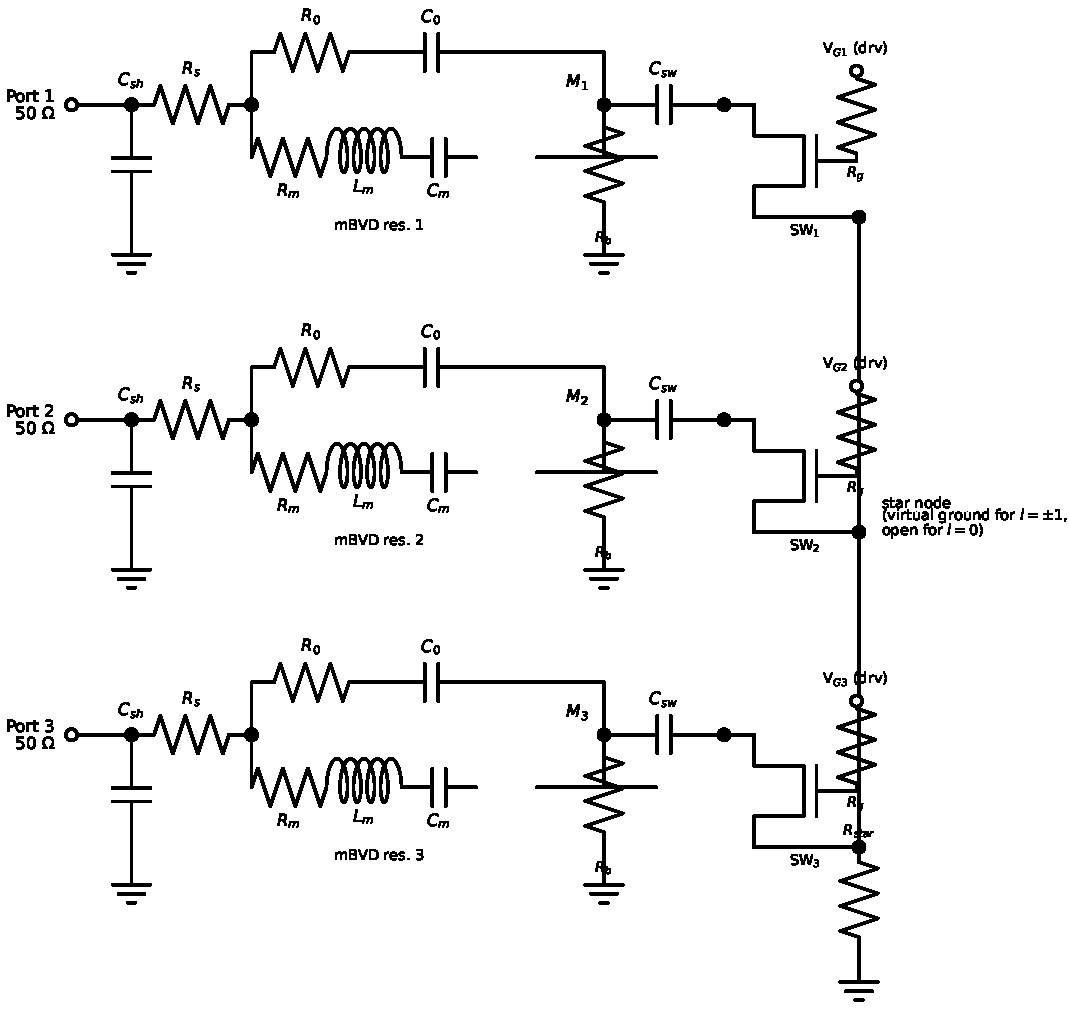
\includegraphics[width=\columnwidth]{fig_schematic_core}
\caption{Circulator core: three mBVD LiNbO$_3$ resonators in a series-mode resonant junction. Each branch is modulated by a MIM capacitor $C_{sw}$ in series with a wide nMOS switch SW$_n$ whose gate is driven with phase $0$, \ang{120} or \ang{240}; $C_{sh}$ matches the ports; $R_b$ and $R_{star}$ set the d.c.\ levels. Only capacitors, resistors, resonators and transistors are used.}
\label{fig:core}
\end{figure}

\section{CMOS Pump Design}\label{sec:cmos}
\subsection{Three-phase clock generator}
Fig.~\ref{fig:phasegen} shows the phase generator. A three-stage twisted-ring (Johnson) counter clocked at $6f_m$ produces \SI{50}{\percent}-duty outputs delayed by one clock period each; selecting $Q_0$, $Q_2$ and $\overline{Q_1}$ yields phases of exactly \ang{0}, \ang{120} and \ang{240} without analogue phase interpolation, and the phase error is set only by flip-flop delay mismatch. The flip-flops are transmission-gate master--slave cells (Fig.~\ref{fig:dff}) with a NAND in the master loop for an active-low reset, which forces the counter into the valid state 111 and removes the 010/101 lock-up loop of a Johnson counter. Swapping the \ang{120} and \ang{240} outputs reverses the circulation sense (TX/RX swap), which is useful for antenna balancing and calibration. The reference clock is $6f_m=\SI{\fclk}{MHz}$, \num{\clockratio} times below the RF carrier, in contrast with N-path circulators that require clocks at the carrier frequency.

\subsection{Gate drivers}
Each phase drives a five-stage tapered inverter chain (taper $\times3$, Fig.~\ref{fig:driver}) that charges the gate of the switch between \SI{0}{} and $V_{DD}=\SI{1.2}{V}$. The simulated 10--90\,\% rise time is \SI{\trise}{ns} (\SI{\trisepct}{\percent} of the pump period), which makes the capacitance waveform a trapezoid whose fundamental is within \SI{1}{\percent} of the ideal square wave. Because the pump charges only three gates, the dynamic power is $\approx 3\,C_g V_{DD}^2 f_m$ and the simulated pump power including the counter is \SI{\Pmodtot}{mW}.

\begin{figure}[!t]
\centering
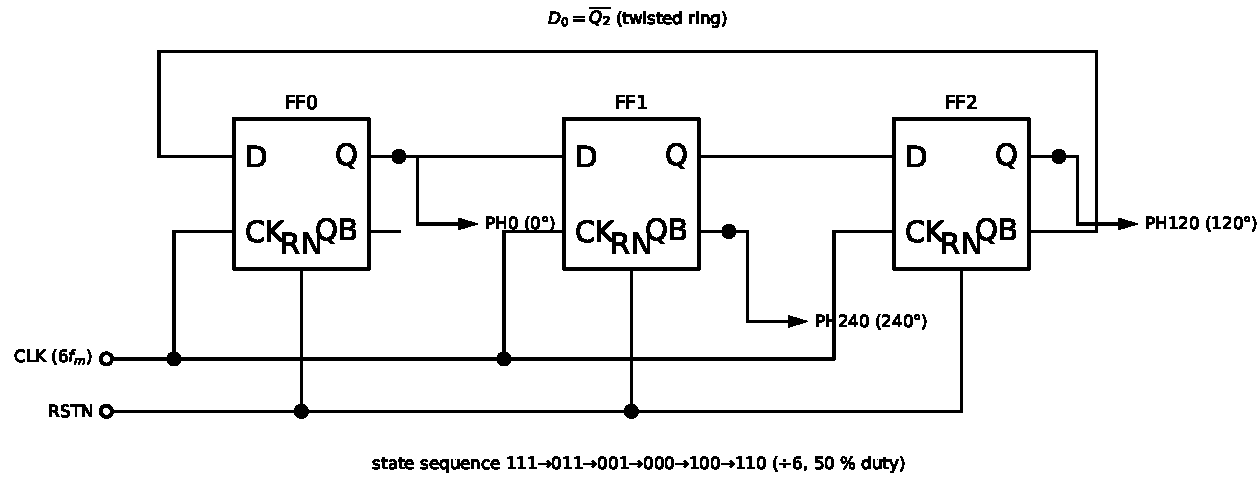
\includegraphics[width=\columnwidth]{fig_schematic_phasegen}
\caption{Divide-by-six Johnson counter generating the three pump phases; the state sequence after reset is shown.}
\label{fig:phasegen}
\end{figure}
\begin{figure}[!t]
\centering
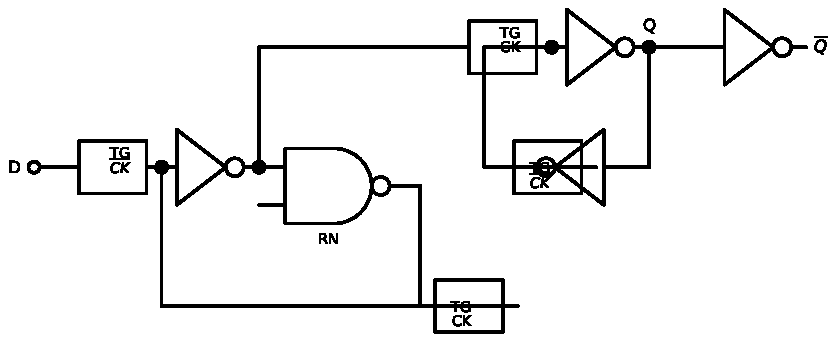
\includegraphics[width=\columnwidth]{fig_schematic_dff}
\caption{Transmission-gate master--slave flip-flop with reset in the master loop.}
\label{fig:dff}
\end{figure}
\begin{figure}[!t]
\centering
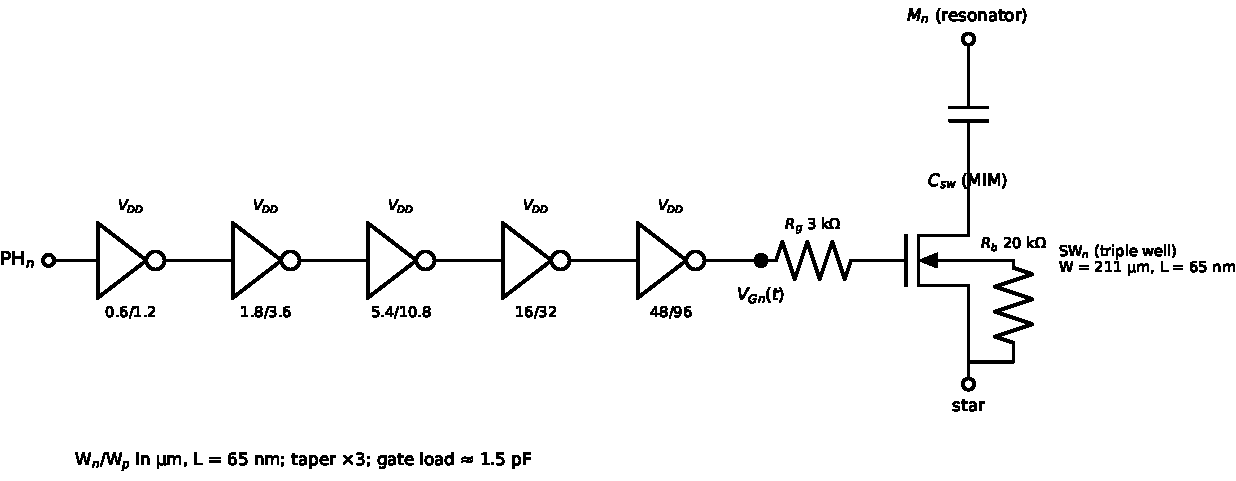
\includegraphics[width=\columnwidth]{fig_schematic_driver}
\caption{Gate driver (tapered inverter chain) and switched MIM modulator. Transistor widths are in \si{\micro\meter}, $L=\SI{65}{nm}$.}
\label{fig:driver}
\end{figure}

\section{Simulation Methodology}\label{sec:method}
Three levels of simulation were used; every number in Section~\ref{sec:results} states which one produced it.

\emph{Floquet CMT} (Section~\ref{sec:theory}) is used for design rules and insight.

\emph{Conversion-matrix periodic S-parameters (LTP/PSP).} The resonator network with its modulated capacitors is a linear time-periodic network. Each modulated capacitor $q=C(t)v$ with $C(t)=\sum_k c_k e^{jk\omega_m t}$ is stamped into a modified nodal analysis matrix as a Toeplitz conversion block $I_m=j(\omega+m\omega_m)\sum_l c_{m-l}V_l$, and each switch as a time-varying conductance $g(t)=\sum_k g_k e^{jk\omega_m t}$ with the block $I_m=\sum_l g_{m-l}V_l$; all time-invariant elements (resonators, MIM capacitors, the off-state capacitance and the residual parasitics of the switches) are block-diagonal across the sidebands, and the system is solved for each port excitation. This is exactly the analysis performed by Spectre's PSS followed by PSP (or HB followed by HBSP). The hard-switched conductance is the physically correct description of a switched capacitor: unlike a varactor, whose capacitance changes losslessly, a MIM capacitor that is connected and disconnected through $R_{on}$ dissipates energy at every switching event, and a model that merely toggles a capacitance value misses this loss (an early version of this work did, and over-estimated the performance by \SI{3}{dB}). Because the conductance jumps by four orders of magnitude, the Fourier series converges slowly, and the shape of the transition matters: the gate voltage is the RC response ($\tau=R_gC_g$) of the square drive and the channel conductance rises linearly above $V_{th}$, which the solver reproduces (waveform `rc'); with this waveform the fundamental-tone S-parameters converge for $K\ge40$ sidebands, which is used for all reported numbers (design-space sweeps use $K=16$ with trapezoidal edges, which is \SI{0.3}{dB} optimistic in insertion loss). The solver was validated against the analytic sideband amplitude of a single modulated capacitor (agreement to \SI{0.01}{dB}), against an ngspice transient of the same element (\SI{0.02}{dB}) and against the CMT in the weak-coupling limit (Fig.~\ref{fig:cmtcheck}). Node voltages are also returned, which gives the voltage stress on the switches as a function of input power.

\begin{figure*}[!t]
\centering
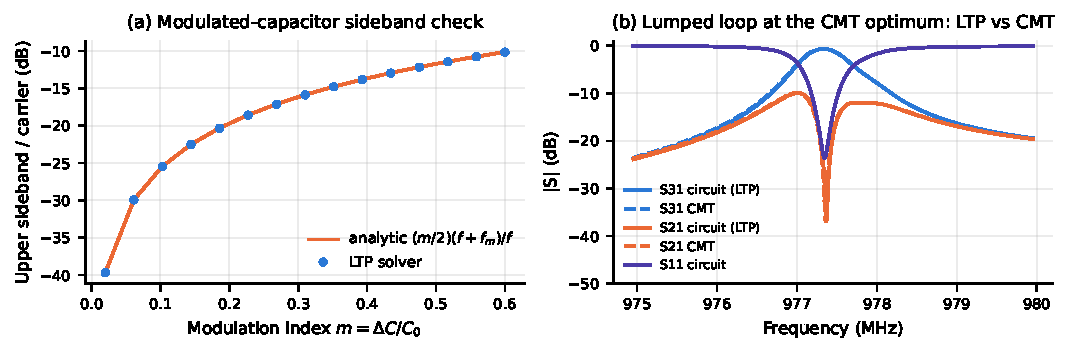
\includegraphics[width=\textwidth]{fig_validation}
\caption{Validation of the conversion-matrix solver: (a) sideband-to-carrier ratio of a single modulated capacitor against the analytic value; (b) ideal lumped three-resonator loop at the CMT optimum of Table~\ref{tab:cmt} ($\omega_m=15\gamma_e$, $|\kappa|=10\gamma_e$, $\Delta\omega=5.6\gamma_e$): circuit solver against CMT.}
\label{fig:cmtcheck}
\end{figure*}

\emph{Transistor-level transient co-simulation.} The complete chip (reference clock, phase generator, drivers, switches, resonator network and \SI{50}{\ohm} ports) is simulated in ngspice~42 with a \SI{65}{nm}-class BSIM4 (level 54) model card in the style of the predictive technology model \cite{zhao2006new}. A single tone is injected at one port, the steady state is Fourier-analysed over an integer number of common periods of the RF and pump frequencies, and $S_{mn}=b_m/a_n$ is formed at the fundamental and at $\omega\pm\omega_m$. Trapezoidal integration is essential: the default Gear integration damps the $Q=500$ resonators numerically and adds \SI{2}{dB} of apparent loss; a \SI{20}{ps} step is within \SI{0.3}{dB} of a \SI{5}{ps} step and is used for the sweeps. This corresponds to the Spectre transient flow (or PSS with the RF tone as a second fundamental); the equivalent Spectre netlists and an OCEAN script that runs PSS+PSP and extracts the same figures of merit are supplied so that the results can be regenerated in Cadence Virtuoso with a foundry PDK.

\emph{Design search.} For each topology and modulator a differential-evolution search over the coupling, modulator and pump variables was run with the operating frequency found adaptively for every candidate (coarse sweep, local refinement), followed by a simplex polish and a re-centring of the resonator $f_s$ so that the operating point sits at \SI{1.000}{GHz}; the pump frequency was then snapped to a \SI{5}{MHz} grid for commensurate transient analysis.

\section{Simulation Results}\label{sec:results}
\subsection{Design point}
Table~\ref{tab:design} lists the design point. Fig.~\ref{fig:unmod} shows the reciprocal junction with the switches held on: the degenerate counter-rotating pair at \SI{\fdeg}{MHz} transmits \SI{\Sunmod}{dB} to each of the other ports with \SI{\Sunmodrl}{dB} return loss, close to the \SI{-3.5}{dB}/\SI{9.5}{dB} of a lossless symmetric three-port, with a loaded $Q$ of \Qload; with the switches held off the junction reflects.

\begin{table}[!t]
\centering
\caption{Design point and simulated performance}
\label{tab:design}
\footnotesize
\begin{tabular}{@{}llc@{}}
\toprule
\multicolumn{3}{l}{\emph{Resonators and passives}}\\
$f_s$ / $f_p$ & \SI{\fs}{} / \SI{\fp}{MHz} & \\
$C_0$, $C_m$, $Q_m$ & \SI{\Cnought}{}, \SI{\Cm}{pF}, \Qm &\\
$C_{sh}$ (per port) & \SI{\Csh}{pF} & MIM\\
$C_{sw}$, $C_{par}$ & \SI{\Csw}{pF}, \SI{\Cpar}{pF} & MIM\\
Switch $W/L$ & \SI{\Wsw}{\micro\meter}/\SI{65}{nm} & nMOS\\
$R_{on}$, $C_{off}$ & \SI{\Ron}{\ohm}, \SI{\Coff}{fF} & \\
\midrule
\multicolumn{3}{l}{\emph{Pump}}\\
$f_m$, $6f_m$ & \SI{\fm}{MHz}, \SI{\fclk}{MHz} & \\
Pump power (drivers $+$ counter) & \SI{\Pmodtot}{mW} & ngspice\\
\midrule
\multicolumn{3}{l}{\emph{Performance at $f_0=\SI{\fop}{GHz}$}}\\
Insertion loss (worst path) & \SI{\ILdB}{dB} & ngspice\\
Isolation (worst path) & \SI{\ISOdB}{dB} & ngspice\\
Return loss (worst port) & \SI{\RLdB}{dB} & ngspice\\
IL / ISO / RL & \SI{\ILltp}{} / \SI{\ISOltp}{} / \SI{\RLltp}{dB} & LTP/PSP\\
Reverse sense IL / ISO & \SI{\revIL}{} / \SI{\revISO}{dB} & LTP/PSP\\
20-dB (15-dB) ISO bandwidth & \SI{\BWiso}{} (\SI{\BWisofifteen}{}) \si{MHz} & LTP/PSP\\
1-dB IL bandwidth & \SI{\BWil}{MHz} & LTP/PSP\\
Sidebands $f{+}f_m$, $f{-}f_m$ (1$\to$2) & \SI{\IMup}{}, \SI{\IMdn}{dBc} & ngspice\\
Pump phases & \SI{\phasetwo}{\degree}, \SI{\phasethree}{\degree} & ngspice\\
$P_{in,\max}$ ($|V_{ds}|<1.2$ V; $2\times$ stack) & \SI{\Pmaxone}{} (\SI{\Pmaxtwo}{}) dBm & LTP\\
\bottomrule
\end{tabular}
\end{table}

\subsection{S-parameters}
Fig.~\ref{fig:sparams} shows the fundamental-tone S-parameters from the LTP/PSP analysis and Fig.~\ref{fig:ngspice} the transistor-level transient results with the real CMOS pump superimposed on the LTP curves. The shapes of all nine S-parameters and of the sideband conversion agree over the band, and the transient confirms circulation with \SI{\ILdB}{dB} insertion loss and \SI{\ISOdB}{dB} isolation at $f_0$ (best isolation \SI{\ngbestiso}{dB} at \SI{\ngbestf}{MHz}). The design model is, however, \SI{\agreeIL}{dB} optimistic in insertion loss and its isolation notch is deeper (\SI{\ISOltp}{dB}); the residual comes from the switch transitions, during which the MOSFET passes through a resistive region whose conductance depends on the instantaneous gate and channel voltages in a way that the linear-ramp conductance of the design model only approximates. We therefore quote the transient values as the performance of the design and use the LTP/PSP model, which is two to three orders of magnitude faster, for synthesis and sensitivity. With an ideal square-wave pump the transient gives \SI{\idealIL}{dB} and \SI{\idealISO}{dB}, so the CMOS phase generator and drivers themselves cost nothing measurable. Circulation is in the sense $1\!\to\!2\!\to\!3\!\to\!1$; swapping the \ang{120} and \ang{240} phases reverses it with identical performance (Table~\ref{tab:design}). The dominant spurious response is the lower sideband at $f-f_m$, at \SI{\IMdn}{dBc} (upper sideband \SI{\IMup}{dBc}); it is the main loss mechanism of the hard-switched modulator and, because $f_m$ is derived from the system clock, falls at a known offset where the channel filter removes it.

\begin{figure}[!t]
\centering
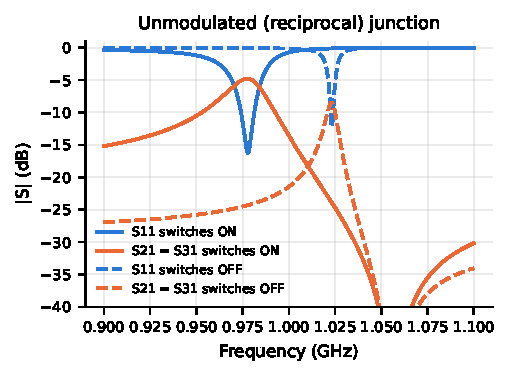
\includegraphics[width=\columnwidth]{fig_unmodulated}
\caption{Unmodulated junction (LTP): switches on (reciprocal three-port with the degenerate $l=\pm1$ pair) and switches off.}
\label{fig:unmod}
\end{figure}
\begin{figure*}[!t]
\centering
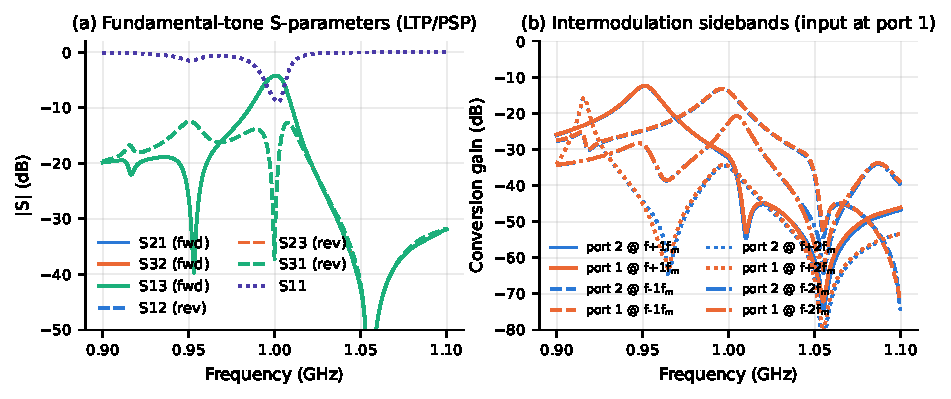
\includegraphics[width=\textwidth]{fig_sparams_ltp}
\caption{(a) Fundamental-tone S-parameters of the modulated junction from the conversion-matrix (PSP-equivalent) analysis: solid, forward paths; dashed, reverse paths; dotted, $S_{11}$. (b) Intermodulation sidebands for an input at port~1.}
\label{fig:sparams}
\end{figure*}
\begin{figure*}[!t]
\centering
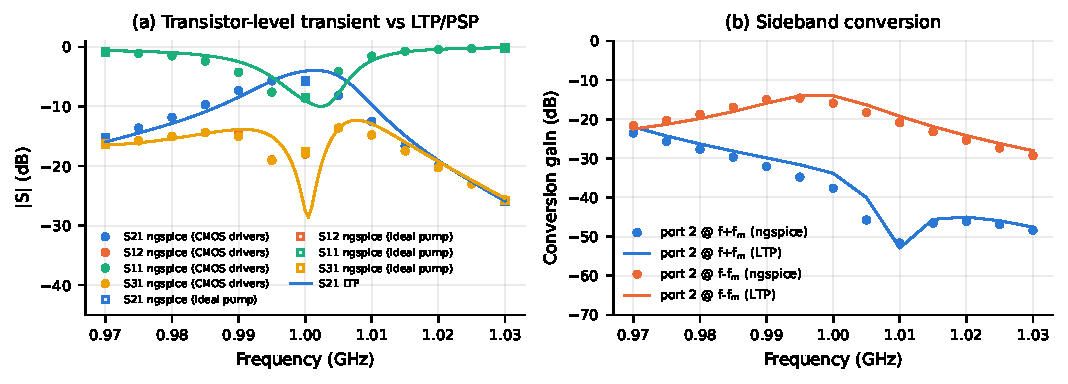
\includegraphics[width=\textwidth]{fig_sparams_ngspice}
\caption{Transistor-level transient co-simulation in ngspice (markers; filled: CMOS phase generator and drivers, open: ideal square-wave pump) compared with the LTP/PSP analysis (lines). (a) $S_{21}$, $S_{12}$, $S_{11}$, $S_{31}$; (b) sideband conversion.}
\label{fig:ngspice}
\end{figure*}

\subsection{Waveforms}
Fig.~\ref{fig:pgwave} shows the reference clock, the Johnson-counter outputs and the driver outputs at the switch gates, and Fig.~\ref{fig:waves} the three gate drives together with the port voltages when a \SI{\fop}{GHz} tone is injected at port~1: the signal appears at port~2 and is suppressed at port~3. The simulated phase spacing is \SI{\phasetwo}{\degree} and \SI{\phasethree}{\degree}, i.e.\ an error below \SI{\phaseerr}{\degree}.

\begin{figure}[!t]
\centering
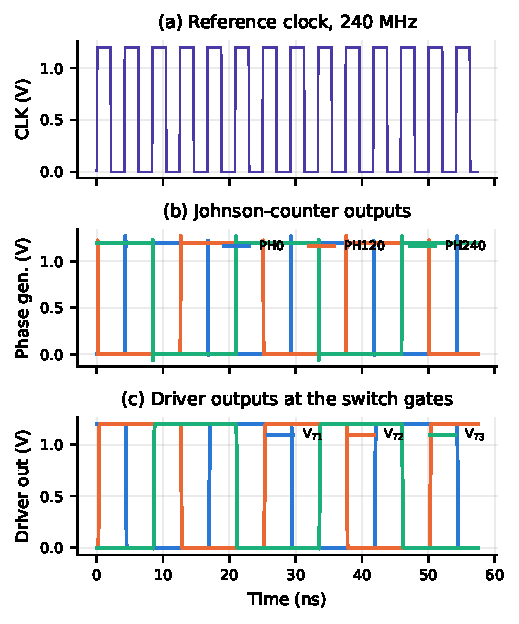
\includegraphics[width=\columnwidth]{fig_phasegen_waveforms}
\caption{ngspice waveforms of the pump: (a) reference clock at $6f_m$, (b) Johnson-counter phases, (c) driver outputs at the switch gates.}
\label{fig:pgwave}
\end{figure}
\begin{figure}[!t]
\centering
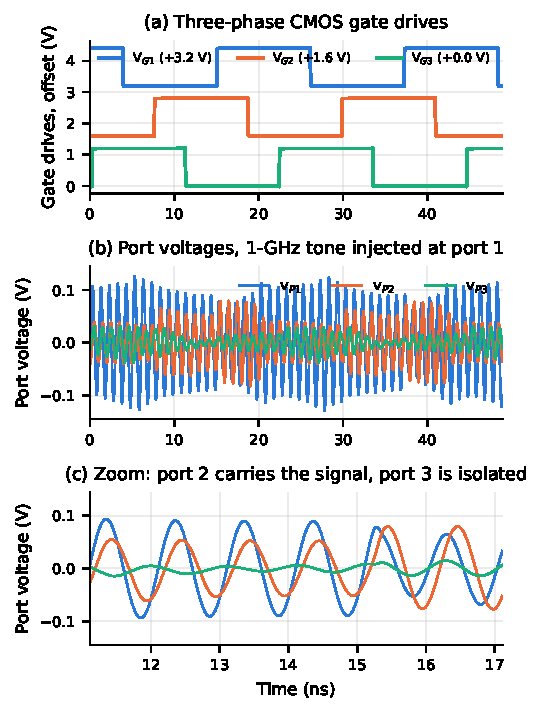
\includegraphics[width=\columnwidth]{fig_waveforms}
\caption{Transistor-level co-simulation: (a) gate drives, (b) port voltages for a tone at port~1, (c) zoom showing transmission to port~2 and isolation of port~3.}
\label{fig:waves}
\end{figure}

\subsection{Eigenmode picture and CMT consistency}
Fig.~\ref{fig:modes} shows the reflection coefficients of the three eigen-excitations of the junction, $\Gamma_l=S_{11}+S_{21}e^{j2\pi l/3}+S_{31}e^{-j2\pi l/3}$, with the switches held on and off. The in-phase excitation ($l=0$) is totally reflected in both states ($|\Gamma_0|=1$, phase \SI{\gzerophase}{\degree} at $f_0$) and shows no resonance, which is the non-resonant $l=0$ mode of Section~\ref{sec:arch}. The counter-rotating excitation ($l=\pm1$) is resonant: a single-pole CMT fit gives, with the switches on, $f_{\pm1}=\SI{\fonres}{MHz}$, $\gamma_e/2\pi=\SI{\geon}{MHz}$ and $\gamma_i/2\pi=\SI{\gion}{MHz}$ ($Q_e=\Qeon$, $Q_i=\Qion$), and with the switches off the counter-rotating resonance moves to \SI{\foffres}{MHz}, \SI{\detoff}{MHz} higher, where the branch is much more weakly coupled (reflection dip of only \SI{\goffmin}{dB}). The two-state modulation therefore switches the counter-rotating pair between a well-coupled and a detuned, weakly coupled state; in the language of (\ref{eq:mod}) it is a square-wave frequency modulation of amplitude $\approx\pm\SI{\detoffhalf}{MHz}$ accompanied by a modulation of the coupling. The loss ratio of the on state, $\gamma_i/\gamma_e=\num{\lossratioon}$, corresponds on the CMT loss curve of Section~\ref{sec:theory} to an insertion loss of \SI{\cmtilpred}{dB}; the circuit value of \SI{\ILltp}{dB} is slightly better because the junction spends part of the pump period in the lower-loss off state. The insertion loss of the design is thus loss-limited, as (\ref{eq:fom}) predicts, and the figure of merit identifies the levers: resonator $Q_m$ and switch $R_{on}W$.

\begin{figure*}[!t]
\centering
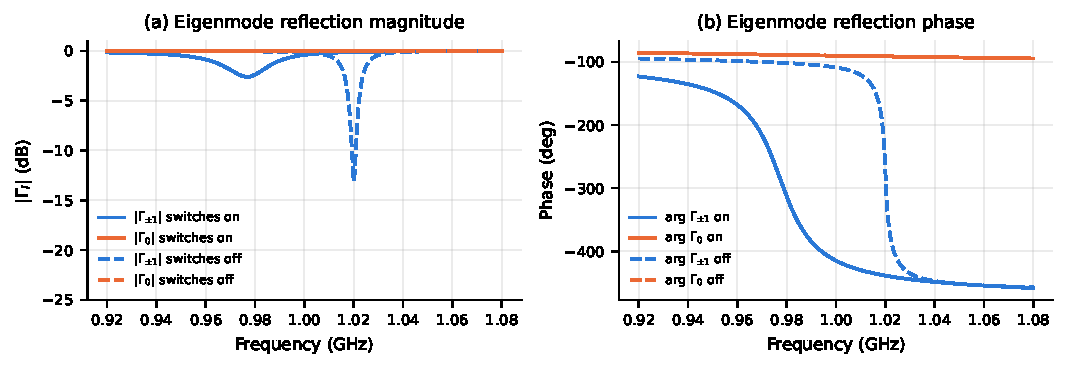
\includegraphics[width=\textwidth]{fig_junction_modes}
\caption{Eigenmode reflection coefficients of the unmodulated junction (LTP) for the in-phase ($l=0$) and counter-rotating ($l=\pm1$) excitations with the switches on and off: (a) magnitude, (b) phase.}
\label{fig:modes}
\end{figure*}

\subsection{Design space, projections and sensitivity}
Fig.~\ref{fig:space} sweeps the design around the design point. (a) The switch width trades $R_{on}$ (insertion loss) against the off-state capacitance and the gate charge (modulation depth, edge speed and return loss). (b) $C_{sw}$ sets the branch resonance and the tuning share $C_m/C_v$. (c) The pump frequency behaves as in Table~\ref{tab:cmt}: the insertion loss improves slowly with $f_m$ while the isolation bandwidth narrows. (d) The resonator $Q_m$ enters through $Q_t$ in (\ref{eq:fom}). Table~\ref{tab:proj} projects the performance for resonator and switch improvements with the design otherwise unchanged; a lower $R_{on}W$ alone does not help because the switch width was already chosen for the given $R_{on}W$, whereas the resonator $Q_m$ acts directly on the loss ratio: with $Q_m=1000$ (demonstrated for SH0 LiNbO$_3$ resonators below \SI{1}{GHz} \cite{lu2018lithium}) the insertion loss drops to \SI{\projILq}{dB}, and with $Q_m=2000$ and a switch with $R_{on}W=\SI{120}{\ohm\micro\meter}$ to \SI{\projILbest}{dB}. Fig.~\ref{fig:mismatch}(a) shows that finite gate edges up to \SI{10}{\percent} of the period are harmless, and Fig.~\ref{fig:mismatch}(b) the sensitivity to a phase error of one pump channel or a mismatch of one $C_{sw}$: isolation stays above \SI{\tolfloor}{dB} for phase errors up to \SI{\phasetol}{\degree} and capacitor mismatch up to \SI{\cswtol}{\percent}; the digital phase generator is far more accurate than the former, and the latter is within MIM matching for a few-pF capacitor, with a per-branch trim available through $C_{par}$.

\begin{figure*}[!t]
\centering
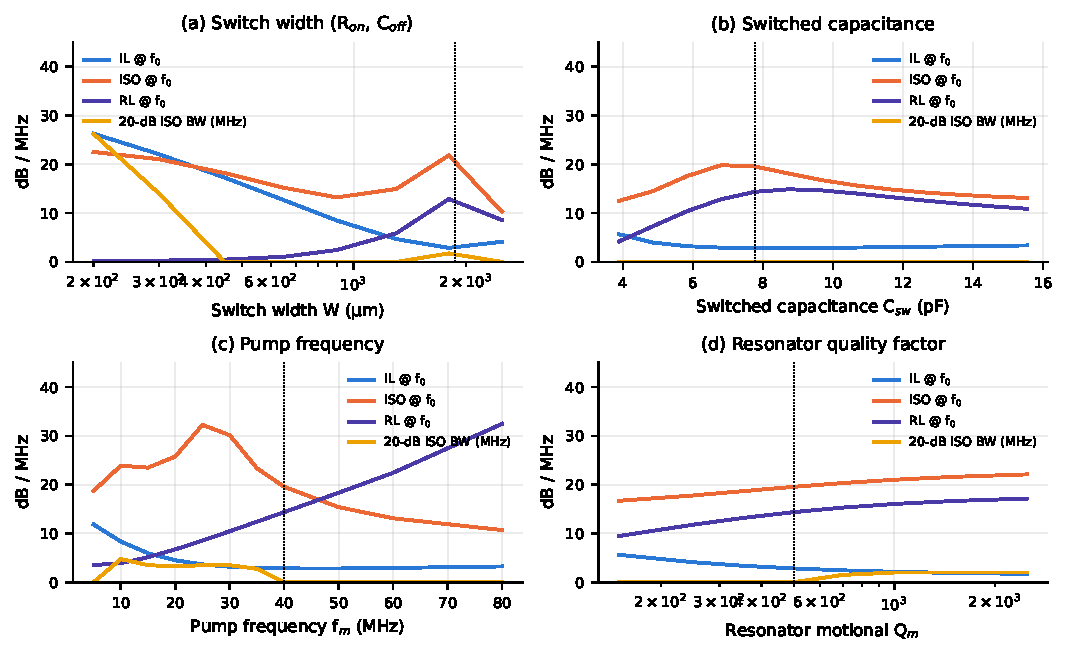
\includegraphics[width=\textwidth]{fig_design_space}
\caption{Design-space sweeps (LTP): (a) switch width, (b) switched capacitance, (c) pump frequency, (d) resonator $Q_m$. Dotted lines mark the design point.}
\label{fig:space}
\end{figure*}
\begin{figure*}[!t]
\centering
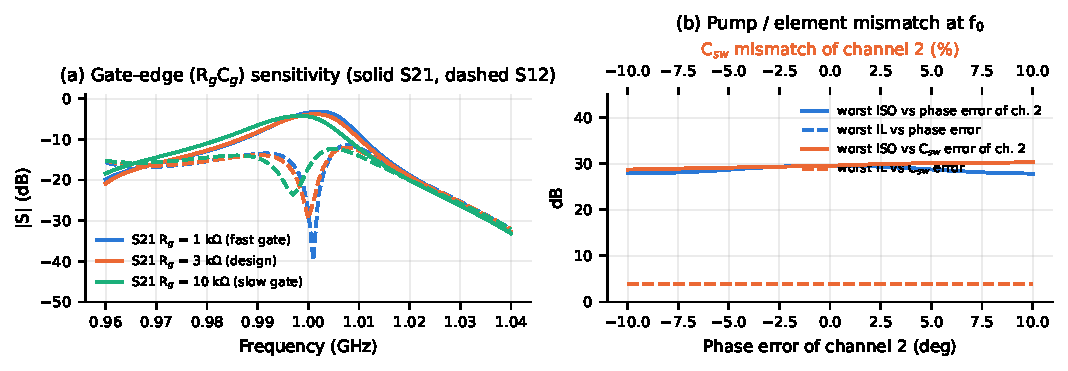
\includegraphics[width=\textwidth]{fig_waveform_mismatch}
\caption{(a) Sensitivity to the switching-edge duration. (b) Sensitivity to a phase error of one pump channel and to a mismatch of one $C_{sw}$.}
\label{fig:mismatch}
\end{figure*}

\begin{table}[!t]
\centering
\caption{Projection with resonator and switch quality (LTP, design point otherwise unchanged)}
\label{tab:proj}
\scriptsize\setlength{\tabcolsep}{2.5pt}
\begin{tabular}{S[table-format=4.0] S[table-format=3.0] S[table-format=1.2] S[table-format=2.1] S[table-format=2.1] S[table-format=1.0]}
\toprule
{$Q_m$} & {$R_{on}W$} & {IL} & {ISO} & {RL} & {BW$_{15}$}\\
 & {(\si{\ohm\micro\meter})} & {(dB)} & {(dB)} & {(dB)} & {(MHz)}\\
\midrule
\projrows
\bottomrule
\end{tabular}
\end{table}

\subsection{Topology and modulator comparison}
Table~\ref{tab:topo} summarises the global searches (same resonator, $Q_m=500$). The parallel-mode loop does not circulate for the reasons given in Section~\ref{sec:arch}; the series-mode junction circulates with both modulators. The varactor row is computed with the lossless-modulation (time-varying capacitance) model that is exact for a varactor, the switched-MIM rows with the hard-switched conductance model; the switched MIM capacitor is better by \SI{\swgain}{dB} of insertion loss while needing an order of magnitude less pump power and no bias network inside the junction.

\begin{table}[!t]
\centering
\caption{Topology / modulator comparison (LTP, global search, $Q_m=500$ unless stated)}
\label{tab:topo}
\scriptsize\setlength{\tabcolsep}{3pt}
\begin{tabular}{llS[table-format=1.2]S[table-format=2.1]S[table-format=2.1]S[table-format=2.1]}
\toprule
Topology & Modulator & {IL (dB)} & {ISO (dB)} & {RL (dB)} & {$f_m$ (MHz)}\\
\midrule
\toporows
\bottomrule
\end{tabular}
\end{table}

\subsection{Power handling}
From the LTP node voltages, the peak voltage across the switch of the excited branch is \num{\vdspkpervolt}~V per volt of source amplitude at $f_0$. Keeping $|V_{ds}|$ below \SI{1.2}{V} limits the input power to \SI{\Pmaxone}{dBm} for a single switch and \SI{\Pmaxtwo}{dBm} for a two-transistor stack, which the transient co-simulation confirms (\SI{\vdspk}{V} peak at \SI{\Pinng}{dBm}). This is adequate for IoT-class and short-range full-duplex links; higher power needs thick-oxide or stacked switches with the usual $R_{on}$ penalty, which (\ref{eq:fom}) converts directly into insertion loss.

\subsection{Comparison with the state of the art}
Table~\ref{tab:soa} places the design among magnet-free circulators. Its distinguishing features are the absence of inductors and of carrier-rate clocks: the pump is \num{\clockratio} times below the carrier and consumes \SI{\Pmodtot}{mW}, two orders of magnitude below N-path CMOS circulators. The isolation bandwidth is narrow, as for all resonant STM circulators, and matches narrow-band IoT and sensing full-duplex links rather than wideband cellular carriers; the insertion loss is set by (\ref{eq:fom}) and improves directly with resonator $Q$ and switch quality.

\begin{table*}[!t]
\centering
\caption{Comparison with reported magnet-free circulators$^{\dagger}$}
\label{tab:soa}
\footnotesize\setlength{\tabcolsep}{2.5pt}
\begin{tabular}{lllllllll}
\toprule
Ref. & Principle & Technology & $f_0$ & Pump/clock & IL (dB) & ISO (dB) & Pump power & Inductors\\
\midrule
\cite{reiskarimian2017cmos} & N-path commutation & 65 nm CMOS & 0.75 GHz & $f_0$ (8 phases) & 1.7 & 42$^{\ddagger}$ & 59 mW & yes (on-chip)\\
\cite{dinc2017millimeter} & Conductivity mod. & 45 nm SOI & 25 GHz & $f_0/3$ & 3.3 & 18--20 & 78 mW & T-lines\\
\cite{nagulu2019nonmagnetic} & Switched T-line & 65 nm CMOS & $\approx$1 GHz & $f_0$ & $\approx$2 & $>$20 & tens of mW & T-lines\\
\cite{estep2014magnetic} & STM resonator loop & PCB, varactors & 0.17 GHz & $\ll f_0$ & $\approx$2 & $>$20 & n/r & yes\\
\cite{kord2018magnetless} & STM bandstop delta & PCB, varactors & $\approx$1 GHz & $\ll f_0$ & $\approx$3 & $>$30 & n/r & yes\\
\cite{torunbalci2018fbar} & Commutated FBAR & FBAR, ext. switches & 2.5 GHz & $\ll f_0$ & n/r & n/r & external & no\\
\cite{yu2019radio} & STM SAW filters & SAW + ext. pump & 0.1--0.2 GHz & $\ll f_0$ & n/r & n/r & external & no\\
This work (sim.) & STM acoustic junction & LiNbO$_3$, 65 nm CMOS & \SI{\fop}{GHz} & $f_0/\num{\clockratio}$ & \ILdB & \ISOdB & \SI{\Pmodtot}{mW} & no\\
\bottomrule
\multicolumn{9}{l}{\footnotesize $^{\dagger}$Prior-work values quoted from the cited papers to the best of the author's reading; check against the originals before submission. n/r: not reproduced here.}\\
\multicolumn{9}{l}{\footnotesize $^{\ddagger}$with antenna-impedance tuning.}
\end{tabular}
\end{table*}

\section{Layout and Cadence Deliverables}\label{sec:layout}
Fig.~\ref{fig:layout} shows the tape-out candidate layout of the CMOS die generated from the design (1P9M, \SI{0.8}{mm}$\times$\SI{0.8}{mm} pad-limited): three modulation channels (gate driver, \SI{\Wsw}{\micro\meter} multi-finger switch, $C_{sw}$ and $C_{sh}$ MIM capacitors) are placed around three flip-chip landing pads for the LiNbO$_3$ resonator die, with the phase generator near the clock pad, ground-signal-ground RF pads on three sides and d.c./clock pads on the fourth. The active area of one channel is \SI{\chanw}{}$\times$\SI{\chanh}{\micro\meter}. The layout uses a generic layer map; design-rule and layout-versus-schematic sign-off must be performed in the target PDK. The design files include Spectre netlists of the core and of the complete chip, an OCEAN script that runs PSS/PSP and extracts IL, isolation, return loss and bandwidth, and a SKILL script that builds the schematic cellviews in a Virtuoso library.

\begin{figure}[!t]
\centering
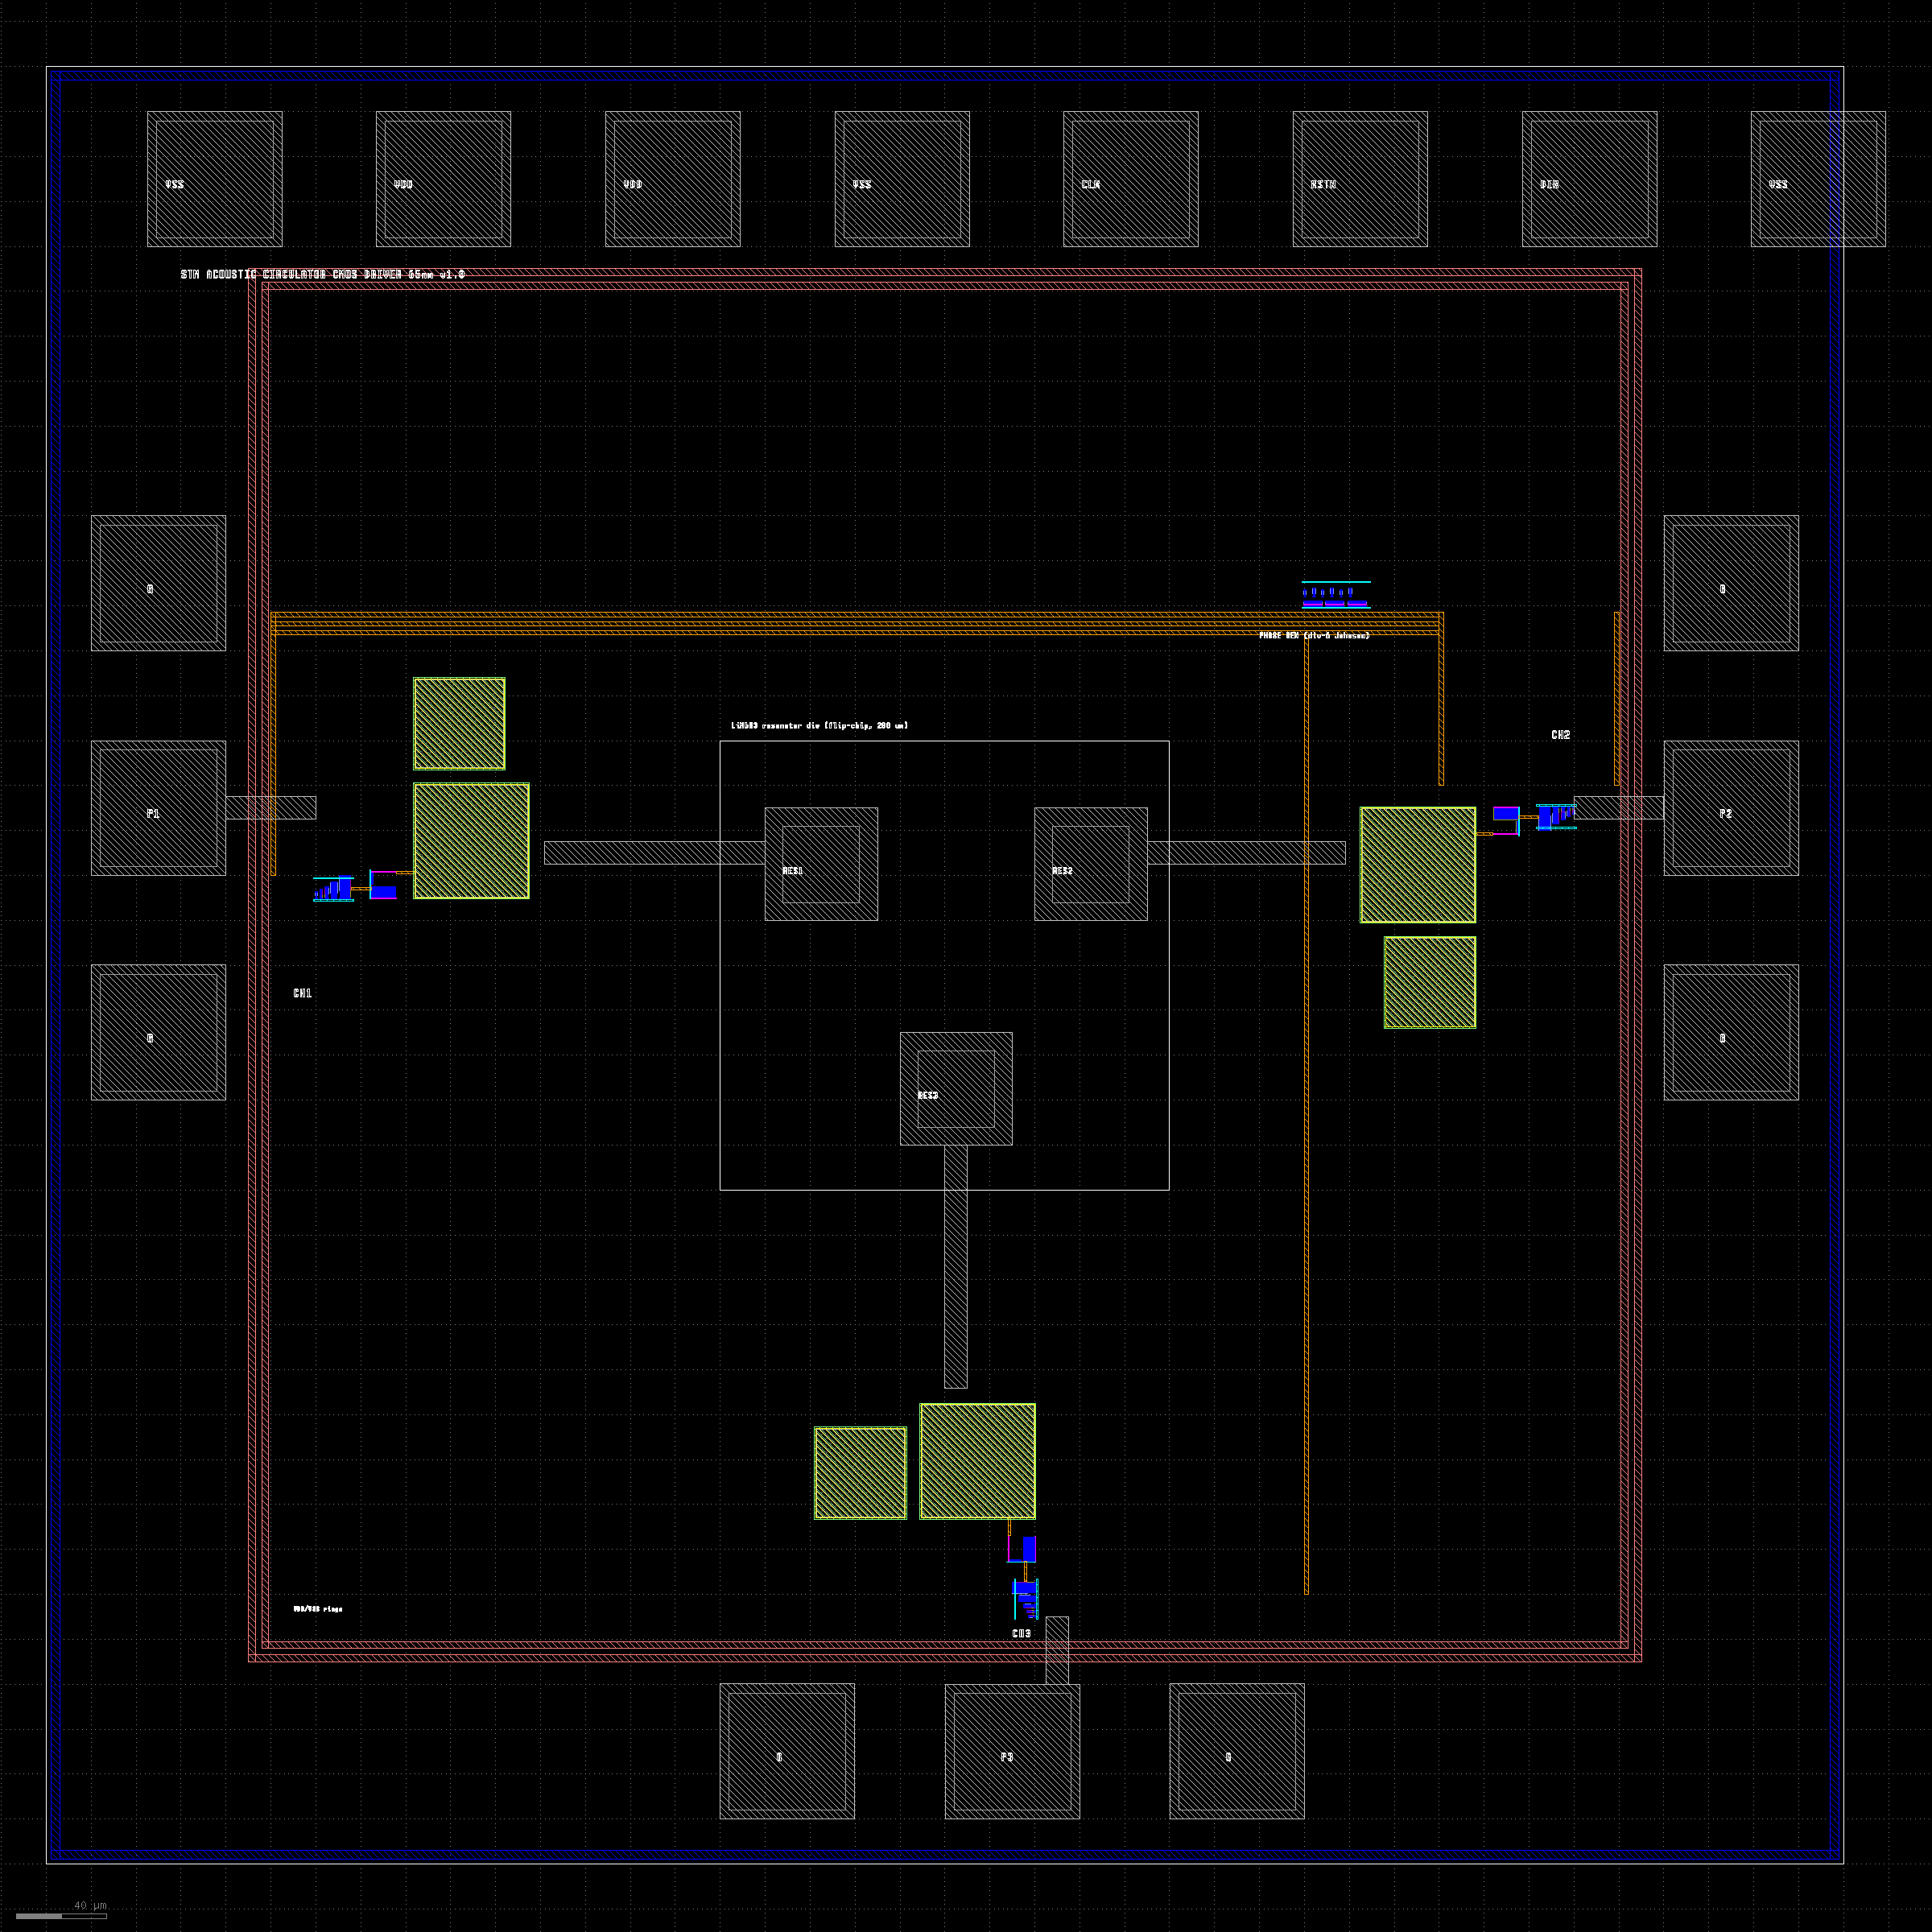
\includegraphics[width=\columnwidth]{fig_layout_top}
\caption{Tape-out candidate layout of the CMOS driver die (generic 65 nm 1P9M layer map, rendered in KLayout): three modulation channels, phase generator, RF GSG pads and flip-chip landing pads for the resonator die.}
\label{fig:layout}
\end{figure}

\section{Discussion and Limitations}
\emph{Model fidelity.} The resonator is an mBVD model with literature-representative parameters; spurious modes, temperature drift (LiNbO$_3$: about \SI{-80}{ppm/K}) and resonator-to-resonator mismatch are not included. Mismatch between the three branches is the dominant practical risk for any STM circulator; the sensitivity analysis bounds the tolerable mismatch, and a per-branch trim capacitor $C_{par}$ provides the correction. \emph{Transistor models.} The CMOS blocks use a predictive BSIM4 card; in a foundry PDK the switch $R_{on}W$, $C_{off}$ and the MIM density will change the numbers but not the design procedure, which is why the Cadence scripts are parameterised. \emph{Linearity.} The switch is linear in both states and the MIM capacitors are linear; the residual nonlinearity comes from the off-state junction capacitance and should be quantified with a two-tone PSS/QPSS analysis in Spectre. \emph{Bandwidth.} Being resonant, the device has a 20-dB isolation bandwidth of \SI{\BWiso}{MHz}; bandwidth extension techniques for cyclic-symmetric STM circulators \cite{kord2018broadband} apply directly. \emph{Insertion loss.} At \SI{\ILdB}{dB} the loss is higher than that of the best N-path CMOS circulators, but (\ref{eq:fom}) and Table~\ref{tab:proj} show that it is a component-quality limit rather than an architectural one, and that it is reached with a pump power two orders of magnitude lower. The two levers are the resonator $Q_m$ (Table~\ref{tab:proj}) and the switching loss, which a soft-switching gate waveform or a varactor with a lossless bias path would remove; both are circuit-level problems rather than physics limits.

\section{Conclusion}
A CMOS-driven, inductor-less, magnet-free acoustic circulator has been designed and verified at circuit and transistor level. A Floquet coupled-mode theory provides closed-form design rules and identifies the tunability--quality-factor product $Q_t\Delta f/f_0$ as the figure of merit that governs insertion loss; circuit-exact analysis shows that the classical capacitively coupled resonator loop cannot be built with acoustic resonators and that a series-mode resonant junction with switched MIM modulators can. A \SI{65}{nm} divide-by-six Johnson counter and tapered gate drivers pump three LiNbO$_3$ resonators at \SI{\fm}{MHz}, \num{\clockratio} times below the \SI{\fop}{GHz} carrier, with \SI{\Pmodtot}{mW}. The transistor-level simulation of the device gives \SI{\ILdB}{dB} insertion loss and \SI{\ISOdB}{dB} isolation at \SI{\fop}{GHz}; the figure of merit shows that the loss is set by the resonator $Q$ and by the switching loss of the modulator, and the projections quantify the component quality needed for the \SI{1}{dB} class. The provided Spectre, OCEAN, SKILL and GDSII files allow the design to be ported to a foundry PDK, taped out and measured, which is the necessary next step.

\section*{Acknowledgment}
The author thanks the open-source EDA community for ngspice and KLayout.

\bibliographystyle{IEEEtran}
\bibliography{refs}

\end{document}
